\section{The model}
\label{sec:model}

This section sets out the blocks of OG-Core following \citet{DeBackerEvans2024}, in the configuration used by the PolicyEngine Macro integration: a single production sector, and households differentiated by age and lifetime ability. Relative to the compact statement in earlier drafts, this section derives the household first-order conditions step by step, motivates the elliptical disutility of labour against the constant-Frisch-elasticity (CFE) alternative, derives the firm conditions under the corporate tax wedge, states the full government block including every fiscal closure rule the framework supports, and describes the demographic machinery and the two solution algorithms with their convergence criteria.

Time is annual. Households live at most $E+S$ periods: $E$ economically inactive childhood years (ages 0--19) and $S=80$ active years (model ages $s = E+1,\dots,E+S$, real ages 20--99). Each cohort contains $J$ lifetime-ability types indexed by $j$, with population shares $\lambda_j$ ($\sum_j \lambda_j = 1$) and deterministic age--ability effective-labour profiles $e_{j,s}$. Population $\omega_{s,t}$ evolves by exogenous fertility, mortality $\rho_s$, and immigration (Section~\ref{subsec:demographics}); labour-augmenting productivity grows at rate $g_y$, and all equations below are expressed before stationarisation (Section~\ref{subsec:stationarisation}).

\subsection{Demographics}
\label{subsec:demographics}

The demographic block is exogenous to the equilibrium but is the engine of the model's long-run dynamics, so we state it in full. Let $\omega_{s,t}$ denote the number of individuals of age $s\in\{1,\dots,E+S\}$ alive at time $t$, $f_s$ the age-specific fertility rate (births per person of age $s$ per year), $\rho_s$ the age-specific mortality hazard (probability of dying between ages $s$ and $s+1$, with $\rho_{E+S}=1$ imposed so that no one outlives the model), and $i_s$ the age-specific net immigration rate expressed as a fraction of the existing age-$s$ population. The population laws of motion are
\begin{align}
\label{eq:popbirths}
\omega_{1,t+1} &\;=\; (1-\rho_0)\sum_{s=1}^{E+S} f_s\,\omega_{s,t} \;+\; i_1\,\omega_{1,t},\\
\label{eq:popaging}
\omega_{s+1,t+1} &\;=\; (1-\rho_s)\,\omega_{s,t} \;+\; i_{s+1}\,\omega_{s+1,t},
\qquad 1 \le s \le E+S-1 ,
\end{align}
where $\rho_0$ is infant mortality. Equation \eqref{eq:popbirths} says next year's newborns are this year's births that survive infancy plus net child migration; equation \eqref{eq:popaging} says each cohort ages one year, shrinks by mortality, and is augmented by net migration into its age cell.

\paragraph{Data and the immigration residual.} OG-UK populates $\{f_s, \rho_s, \omega_{s,t}\}$ from the United Nations World Population Prospects single-year-of-age series for the United Kingdom \citep{UNWPP2024}, retrieved through the UN Data Portal API with a local CSV fallback shipped in the package (population, fertility, deaths, and infant mortality by single year of age; Figure~\ref{fig:demographics} plots the three inputs). Immigration rates $i_s$ are not taken from a migration series directly; they are computed as the \emph{residual} that reconciles two successive observed population vectors given observed fertility and mortality --- solving \eqref{eq:popbirths}--\eqref{eq:popaging} for $i_s$ given $(\omega_{\cdot,t},\omega_{\cdot,t+1},f_s,\rho_s)$ and averaging over recent year pairs. This guarantees the model's near-term population path tracks the official projection exactly, at the cost of attributing any residual measurement noise to migration.

\begin{figure}[t]
\centering
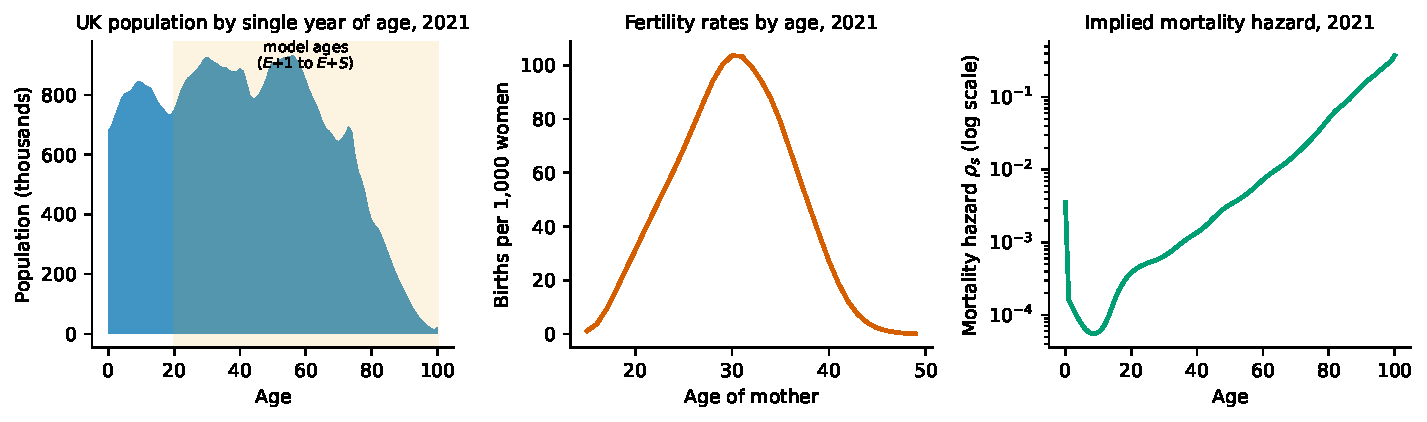
\includegraphics[width=\textwidth]{figures/fig_demographics.pdf}
\caption{Demographic inputs to OG-UK, from the UN World Population Prospects single-year-of-age series for the United Kingdom shipped with the \texttt{oguk} package \citep{UNWPP2024}. Left: population by single year of age (2021), with the model's economically active ages 20--99 shaded. Centre: fertility rates by age of mother. Right: the implied mortality hazard $\rho_s$ (deaths divided by population, log scale), which enters both the households' effective discount factor and the warm-glow bequest weight.}
\label{fig:demographics}
\end{figure}

\paragraph{Transition to a stationary population.} A steady state requires a time-invariant population age distribution. The framework therefore constructs the population path in three phases: (i) for the first $\approx$50 transition periods, the raw laws of motion \eqref{eq:popbirths}--\eqref{eq:popaging} run forward from the current observed age distribution; (ii) the age distribution is then linearly interpolated towards the stationary distribution implied by fixed $(f_s,\rho_s,i_s)$ --- the normalised Perron eigenvector of the linear map defined by \eqref{eq:popbirths}--\eqref{eq:popaging}, whose dominant eigenvalue is one plus the stationary population growth rate $\bar{g}_n$; and (iii) from period $T$ onward the distribution is exactly stationary. The economically active shares used by the equilibrium are the normalised $\hat{\omega}_{s,t} = \omega_{s,t}/\sum_{u=E+1}^{E+S}\omega_{u,t}$ over model ages, and the period-$t$ population growth rate $g_{n,t}$ enters the stationarised resource constraint and the capital-market clearing condition below. The ageing embedded in the UK projection --- a rising old-age share for the next several decades --- is thus an input the steady state inherits, not an assumption bolted on.

\subsection{Households}
\label{subsec:households}

A household of type $j$ and age $s$ at time $t$ has period utility that is additively separable in consumption $c_{j,s,t}$, labour $n_{j,s,t}$, and bequests-to-be-left $b_{j,s+1,t+1}$:
\begin{equation}
\label{eq:utility}
u(c_{j,s,t},n_{j,s,t},b_{j,s+1,t+1}) \;=\; \frac{c_{j,s,t}^{\,1-\sigma}-1}{1-\sigma}
\;+\; e^{g_y t(1-\sigma)}\,\chi^n_s\, v(n_{j,s,t})
\;+\; \chi^b_j\,\rho_s\,\frac{b_{j,s+1,t+1}^{\,1-\sigma}-1}{1-\sigma},
\end{equation}
where $\sigma$ is the coefficient of relative risk aversion, $\chi^n_s$ is an age-specific disutility-of-labour scale, and the warm-glow bequest term is weighted by the mortality hazard $\rho_s$ and an ability-specific intensity $\chi^b_j$ --- a ``joy of giving'' motive in the tradition of \citet{DeNardi2004}, scaled by the probability that the bequest is actually left this period. The factor $e^{g_y t(1-\sigma)}$ on the labour term keeps the consumption--leisure trade-off stable along the balanced-growth path: consumption grows at rate $g_y$ while the time endowment does not, so without this scaling the marginal-utility ratio would trend and hours would drift.

\subsubsection{Elliptical disutility of labour, and why not CFE}
\label{subsubsec:ellipse}

The workhorse specification in the quantitative literature is the constant-Frisch-elasticity (CFE) form
\begin{equation}
\label{eq:cfe}
v_{\text{CFE}}(n) \;=\; -\,\frac{n^{1+\frac{1}{\theta}}}{1+\frac{1}{\theta}},
\qquad v_{\text{CFE}}'(n) \;=\; n^{1/\theta},
\end{equation}
whose Frisch elasticity of labour supply is the constant $\theta$ at every interior point. Its computational defect in a life-cycle model is at the boundaries: $v'_{\text{CFE}}(0)=0$, so nothing in the preferences stops the optimiser from choosing $n\le 0$ for cohorts whose after-tax wage is low (the very old, the low-ability types), and nothing stops $n$ exceeding the time endowment $\tilde{l}$ for high-wage cohorts. Handling this properly requires Kuhn--Tucker complementary-slackness conditions at both bounds for every one of the $S\times J$ labour choices --- occasionally binding constraints that turn a smooth root-finding problem into a nonsmooth one and are a well-documented source of solver failure.

OG-Core instead uses the \emph{elliptical} disutility of \citet{EvansPhillips2018}: take the upper-right quadrant of an ellipse in $(n, -v)$ space with horizontal radius $\tilde{l}$,
\begin{equation}
\label{eq:ellipse}
v(n) \;=\; -\,b\left[\,1-\left(\frac{n}{\tilde{l}}\right)^{\upsilon}\right]^{1/\upsilon},
\qquad b,\upsilon>0,
\end{equation}
with marginal disutility
\begin{equation}
\label{eq:ellipsederiv}
v'(n) \;=\; \frac{b}{\tilde{l}}\left(\frac{n}{\tilde{l}}\right)^{\upsilon-1}
\left[\,1-\left(\frac{n}{\tilde{l}}\right)^{\upsilon}\right]^{\frac{1}{\upsilon}-1} .
\end{equation}
For $\upsilon>1$, expression \eqref{eq:ellipsederiv} tends to $0^+$ as $n\to 0$ \emph{slower than any interior CFE schedule near the top} and, crucially, tends to $+\infty$ as $n\to\tilde{l}$: the Inada-type behaviour at the endowment bound means neither constraint ever binds at an optimum, interior first-order conditions are sufficient everywhere, and the Kuhn--Tucker apparatus disappears. The parameters $(b,\upsilon)$ are not free: OG-Core's \texttt{elliptical\_u\_est} module fits them by minimising the squared distance between \eqref{eq:ellipsederiv} and the CFE marginal disutility $n^{1/\theta}$ over an interior grid of $n$ values, given the calibrated Frisch elasticity $\theta$. The fitted ellipse thus \emph{mimics} CFE behaviour where the data live --- interior hours --- while repairing its boundary behaviour (Figure~\ref{fig:ellipse}). With the OG-Core default Frisch elasticity the fit delivers $b\approx 0.573$ and $\upsilon\approx 2.856$.

\begin{figure}[t]
\centering
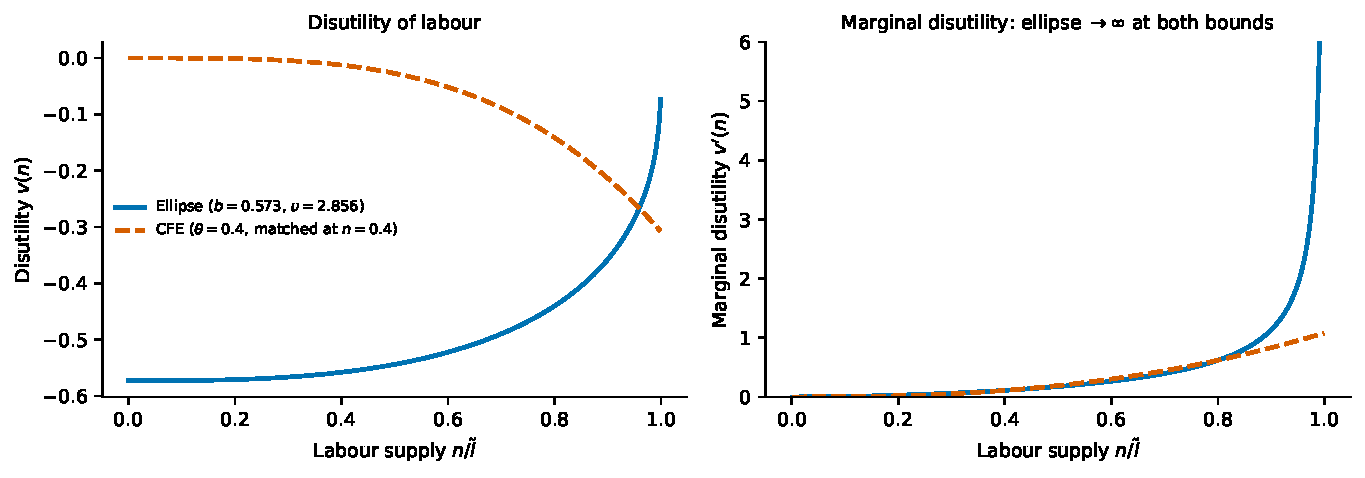
\includegraphics[width=\textwidth]{figures/fig_ellipse.pdf}
\caption{The elliptical disutility of labour \eqref{eq:ellipse} against a CFE specification calibrated to the same Frisch elasticity (scale matched at $n=0.4$), computed from the fitted OG-Core default parameters $(b,\upsilon)$. Left: disutility levels. Right: marginal disutility --- the ellipse tracks CFE over interior hours but its marginal disutility diverges to infinity as $n\to\tilde{l}$ (and its curvature keeps $n>0$), so labour-supply bounds never bind and Kuhn--Tucker conditions are unnecessary \citep{EvansPhillips2018}.}
\label{fig:ellipse}
\end{figure}

\subsubsection{Budget constraint}

The period budget constraint, in the single-good configuration used here (suppressing the multi-good consumption-tax detail of the general framework), is
\begin{equation}
\label{eq:budget}
(1+\tau^c_t)\,c_{j,s,t} + b_{j,s+1,t+1}
\;=\; (1+r_{p,t})\,b_{j,s,t} + w_t\, e_{j,s}\, n_{j,s,t}
+ bq_{j,s,t} + tr_{j,s,t} + pension_{j,s,t} - tax_{j,s,t},
\end{equation}
where $b_{j,s,t}$ is beginning-of-period wealth, $w_t$ is the wage per effective labour unit, $bq_{j,s,t}$ are received bequests, $tr_{j,s,t}$ are government transfers, and $tax_{j,s,t} = \tau^{etr}(x_{j,s,t},y_{j,s,t})\,(x_{j,s,t}+y_{j,s,t})$ is the net income-tax liability generated by the effective-tax-rate function of Section~\ref{sec:taxfunc}, evaluated at labour income $x_{j,s,t}\equiv w_t e_{j,s} n_{j,s,t}$ and capital income $y_{j,s,t}\equiv r_{p,t} b_{j,s,t}$. Two prices deserve comment. The household's return $r_{p,t}$ is the return on a \emph{portfolio}: households hold both private capital and government bonds in proportion to their aggregate supplies, so
\begin{equation}
\label{eq:rport}
r_{p,t} \;=\; \frac{r_t\,K_t + r_{gov,t}\,D_t}{K_t + D_t},
\end{equation}
where $r_t$ is the after-corporate-tax return on capital from the firm block and $r_{gov,t}$ is the government borrowing rate of Section~\ref{subsec:government}. Accidental bequests --- the wealth of those who die, $\sum_s \rho_s\,\omega_{s,t}\,\lambda_j\,b_{j,s+1,t+1}$ --- are redistributed lump-sum within the same ability type $j$ (the deployed configuration; the framework also supports redistribution across types by a fixed matrix), so $bq_{j,s,t}$ is the type-$j$ per-capita share of aggregate type-$j$ bequests $BQ_{j,t}$.

\subsubsection{The household problem and first-order conditions, step by step}
\label{subsubsec:hhfocs}

A household entering economic life at time $t$ chooses $\{c_{j,s,u},n_{j,s,u},b_{j,s+1,u+1}\}$ over its remaining lifetime to maximise
\begin{equation}
\label{eq:lifetime}
\sum_{u=0}^{S-1}\beta^{u}\Bigl[\textstyle\prod_{v=0}^{u-1}(1-\rho_{E+1+v})\Bigr]\,
u\bigl(c_{j,E+1+u,t+u},\,n_{j,E+1+u,t+u},\,b_{j,E+2+u,t+u+1}\bigr),
\end{equation}
subject to the sequence of budget constraints \eqref{eq:budget}, where $\beta$ is the pure discount factor and the product of survival probabilities is the probability of being alive to enjoy period-$u$ utility. There is no aggregate or idiosyncratic risk beyond mortality, and annuity markets are absent (hence accidental bequests). Substitute the budget constraint into \eqref{eq:lifetime} to eliminate $c_{j,s,t}$, or equivalently attach multiplier $\mu_{j,s,t}$ to each period's constraint; we take the Lagrangian route for transparency.

\paragraph{Step 1: marginal utility of wealth.} Differentiating the Lagrangian with respect to $c_{j,s,t}$ gives
\begin{equation}
\label{eq:foc_c}
(c_{j,s,t})^{-\sigma} \;=\; (1+\tau^c_t)\,\mu_{j,s,t},
\end{equation}
so the multiplier is the marginal utility of consumption deflated by the consumption-tax wedge.

\paragraph{Step 2: labour supply.} Differentiating with respect to $n_{j,s,t}$: labour raises resources by the after-tax marginal wage. Because $tax$ depends on labour income both through the ETR level and through the ETR's own slope, the relevant derivative is the \emph{marginal} tax rate on labour income,
\begin{equation}
\label{eq:mtrdef}
\tau^{mtrx}_{j,s,t} \;\equiv\; \frac{\partial\, tax_{j,s,t}}{\partial x_{j,s,t}}
\;=\; \tau^{etr} + (x+y)\,\frac{\partial \tau^{etr}}{\partial x},
\end{equation}
which the pipeline of Section~\ref{sec:taxfunc} estimates directly rather than differentiating the fitted ETR (except under Gouveia--Strauss, where the derivative is analytic). The first-order condition is
\begin{equation}
\label{eq:eul_labor_raw}
w_t e_{j,s}\bigl(1-\tau^{mtrx}_{j,s,t}\bigr)\,\mu_{j,s,t}
\;=\; -\,e^{g_y t(1-\sigma)}\,\chi^n_s\, v'(n_{j,s,t}) \cdot(-1),
\end{equation}
and substituting \eqref{eq:foc_c} for the multiplier gives the labour-supply Euler equation
\begin{equation}
\label{eq:eul_labor}
\frac{w_t e_{j,s}\bigl(1-\tau^{mtrx}_{j,s,t}\bigr)}{1+\tau^c_t}\,(c_{j,s,t})^{-\sigma}
\;=\; e^{g_y t(1-\sigma)}\,\chi^n_s\,
\frac{b}{\tilde{l}}\left(\frac{n_{j,s,t}}{\tilde{l}}\right)^{\upsilon-1}
\left[1-\left(\frac{n_{j,s,t}}{\tilde{l}}\right)^{\upsilon}\right]^{\frac{1}{\upsilon}-1}.
\end{equation}
The left side is the utility value of the after-tax, after-consumption-tax real wage; the right side is the elliptical marginal disutility \eqref{eq:ellipsederiv}. This is where the estimated $\tau^{mtrx}$ function bites: a reform that raises marginal rates over some income range rotates this condition for exactly the households whose $(x,y)$ fall in that range.

\paragraph{Step 3: saving.} Differentiating with respect to $b_{j,s+1,t+1}$, which appears in three places --- today's budget constraint (cost: one unit of resources), tomorrow's budget constraint (benefit: principal plus after-tax return, weighted by survival), and today's warm-glow term (benefit: marginal bequest utility, weighted by death) --- gives
\begin{equation}
\label{eq:eul_save_raw}
\mu_{j,s,t} \;=\; \beta(1-\rho_s)\,
\Bigl[1 + r_{p,t+1}\bigl(1-\tau^{mtry}_{j,s+1,t+1}\bigr)\Bigr]\,\mu_{j,s+1,t+1}
\;+\; \chi^b_j\,\rho_s\,(b_{j,s+1,t+1})^{-\sigma},
\end{equation}
where $\tau^{mtry}$ is the marginal rate on capital income defined analogously to \eqref{eq:mtrdef}. Substituting \eqref{eq:foc_c} (and assuming a constant consumption-tax rate across the two periods for readability) yields the consumption--saving Euler equation for $s<E+S$:
\begin{equation}
\label{eq:eul_save}
(c_{j,s,t})^{-\sigma} \;=\; \beta(1-\rho_s)\,
\Bigl[\,1 + r_{p,t+1}\bigl(1-\tau^{mtry}_{j,s+1,t+1}\bigr)\Bigr]\,(c_{j,s+1,t+1})^{-\sigma}
\;+\; (1+\tau^c_t)\,\chi^b_j\,\rho_s\,(b_{j,s+1,t+1})^{-\sigma}.
\end{equation}
The bequest term acts as a mortality-weighted floor on the return to saving: even when survival-weighted future consumption is worth little (old age, high $\rho_s$), assets retain marginal value because they may be bequeathed. This is what keeps end-of-life asset holdings positive and generates the aggregate bequest flow $BQ$.

\paragraph{Step 4: terminal condition.} In the final period of life $s=E+S$, $\rho_{E+S}=1$: there is no survival continuation, and the choice of terminal assets $b_{j,E+S+1,t+1}$ trades consumption directly against the warm glow,
\begin{equation}
\label{eq:terminal}
(c_{j,E+S,t})^{-\sigma} \;=\; (1+\tau^c_t)\,\chi^b_j\,(b_{j,E+S+1,t+1})^{-\sigma},
\end{equation}
which is \eqref{eq:eul_save} evaluated at $\rho_s=1$. Equations \eqref{eq:eul_labor}, \eqref{eq:eul_save} and \eqref{eq:terminal} --- $2S$ nonlinear equations per ability type, given prices and aggregates --- fully characterise household behaviour, and they show precisely where the microdata-estimated tax functions enter: reforms move $\tau^{etr}$, $\tau^{mtrx}$ and $\tau^{mtry}$ across the joint income distribution, and the general equilibrium reprices $w_t$ and $r_t$ in response.

\subsection{Firms}
\label{subsec:firms}

A unit measure of perfectly competitive firms produces the single output with constant-elasticity-of-substitution technology in private capital $K_t$ and effective labour $L_t$ (the deployed configuration switches off public-capital augmentation):
\begin{equation}
\label{eq:ces}
Y_t \;=\; F(K_t,L_t) \;=\; Z_t\Bigl[\,\gamma^{1/\varepsilon} K_t^{\frac{\varepsilon-1}{\varepsilon}}
+ (1-\gamma)^{1/\varepsilon}\bigl(e^{g_y t} L_t\bigr)^{\frac{\varepsilon-1}{\varepsilon}}\Bigr]^{\frac{\varepsilon}{\varepsilon-1}},
\end{equation}
where $Z_t$ is total factor productivity, $\gamma$ is the capital share parameter, and $\varepsilon$ is the elasticity of substitution. In the Cobb--Douglas limit $\varepsilon = 1$, \eqref{eq:ces} reduces to $Y_t = Z_t K_t^{\gamma}\bigl(e^{g_y t}L_t\bigr)^{1-\gamma}$.

Firms face a corporate income tax at rate $\tau^b_t$ on revenue net of labour costs, with a deduction for depreciation at the \emph{tax} depreciation rate $\delta^\tau_t$ (which may differ from economic depreciation $\delta$ --- capital allowances such as full expensing correspond to $\delta^\tau > \delta$). Firms rent capital at $r_t + \delta$ (the household's required return plus replacement of depreciation) and choose $K_t, L_t$ each period to maximise after-tax profits
\begin{equation}
\label{eq:profits}
PR_t \;=\; (1-\tau^b_t)\bigl(Y_t - w_t L_t\bigr) - \bigl(r_t + \delta\bigr)K_t + \tau^b_t\,\delta^\tau_t K_t .
\end{equation}
The problem is static because capital is rented, not owned. Differentiating with respect to $L_t$:
\begin{equation}
\label{eq:focL}
(1-\tau^b_t)\Bigl(\frac{\partial F}{\partial L_t} - w_t\Bigr) = 0
\quad\Longrightarrow\quad
w_t \;=\; \frac{\partial F}{\partial L_t}
\;=\; e^{g_y t}\,Z_t^{\frac{\varepsilon-1}{\varepsilon}}
\Bigl[(1-\gamma)\,\frac{Y_t}{e^{g_y t}L_t}\Bigr]^{1/\varepsilon} .
\end{equation}
Because wages are deductible, the corporate tax does not distort the labour-demand margin: the wage equals the marginal product of labour exactly. Differentiating with respect to $K_t$:
\begin{equation}
\label{eq:focK}
(1-\tau^b_t)\,\frac{\partial F}{\partial K_t} - (r_t+\delta) + \tau^b_t\,\delta^\tau_t = 0
\quad\Longrightarrow\quad
r_t \;=\; (1-\tau^b_t)\,\Bigl[\gamma\,\frac{Y_t}{K_t}\Bigr]^{1/\varepsilon} Z_t^{\frac{\varepsilon-1}{\varepsilon}} - \delta + \tau^b_t\,\delta^\tau_t .
\end{equation}
The corporate tax drives a wedge between the marginal product of capital and the return households receive: a higher $\tau^b$ lowers $r_t$ for given $K_t$, households accumulate less capital, and in the new equilibrium the pre-tax marginal product is higher, output lower, and --- through \eqref{eq:focL} --- wages lower. This is the channel by which corporation-tax incidence falls partly on labour in the long run, a question the OLG member is specifically equipped to quantify. When $\delta^\tau = \delta$ the depreciation deduction exactly compensates for economic depreciation of the tax base; full expensing ($\delta^\tau$ effectively covering the purchase) pushes the system towards a cash-flow tax that leaves the marginal investment undistorted. The corporation-tax rate $\tau^b$ is a structural parameter of the macro model rather than a PolicyEngine parameter; in the integration it is shocked directly through parameter overrides (Section~\ref{sec:implementation}).

\subsection{Government}
\label{subsec:government}

The government levies household income taxes through the estimated tax functions, consumption taxes at rate $\tau^c_t$, wealth taxes if configured (off in the deployed configuration), and the corporate tax; it spends on public consumption $G_t$, non-pension transfers $TR_t$, public infrastructure investment $I_{g,t}$ (off in the deployed configuration), and pensions; and it issues one-period debt $D_t$.

\paragraph{Revenue.} Aggregate revenue sums the household income-tax liabilities generated by the fitted ETR functions, consumption-tax receipts, and business-tax receipts:
\begin{equation}
\label{eq:revenue}
Rev_t \;=\; \underbrace{\sum_{s,j}\omega_{s,t}\lambda_j\,\tau^{etr}(x_{j,s,t},y_{j,s,t})\,(x_{j,s,t}+y_{j,s,t})}_{\text{income taxes}}
\;+\; \underbrace{\tau^c_t\, C_t}_{\text{consumption taxes}}
\;+\; \underbrace{\tau^b_t\bigl(Y_t - w_t L_t\bigr) - \tau^b_t\,\delta^\tau_t K_t}_{\text{business taxes}} .
\end{equation}

\paragraph{Debt and the government interest rate.} Debt is one-period and rolls over at rate $r_{gov,t}$, which the framework allows to differ from the marginal product-based $r_t$ through an affine wedge,
\begin{equation}
\label{eq:rgov}
r_{gov,t} \;=\; \tau_{d,t}\, r_t + \mu_{d,t},
\end{equation}
with scale $\tau_d$ and level $\mu_d$ calibrated so that the model's effective interest rate on government debt matches the observed gilt-implied rate rather than the corporate return. The flow budget constraint is
\begin{equation}
\label{eq:govbc}
D_{t+1} + Rev_t \;=\; (1+r_{gov,t})\,D_t + G_t + TR_t + Pensions_t + I_{g,t}.
\end{equation}

\paragraph{Baseline spending rules.} Along the baseline, non-pension transfers and public consumption follow fixed GDP shares, $TR_t = \alpha_{tr} Y_t$ and $G_t = \alpha_g Y_t$ (and $I_{g,t} = \alpha_I Y_t$ when public investment is on); pensions follow the configured pension rule (the deployed configuration uses OG-Core's notional-defined-contribution/flat options set to approximate the UK state pension as an age-conditioned transfer).

\paragraph{Fiscal closure rules.} Equation \eqref{eq:govbc} does not by itself pin down a stationary debt path: with spending shares fixed and revenue determined by behaviour, debt would generically follow an explosive or degenerate trajectory. Some fiscal instrument must eventually adjust --- the model must be \emph{closed}. OG-Core implements closure with a two-phase rule governed by parameters $(T_{G1}, T_{G2}, \alpha_D, \rho_G)$: before period $T_{G1}$ the baseline rules run untouched (deficits are whatever they are, capturing near-term announced policy); between $T_{G1}$ and $T_{G2}$ the chosen instrument adjusts partially each period, e.g.\ for a spending closure
\begin{equation}
\label{eq:closure}
G_t \;=\; \rho_G\,\alpha_g Y_t \;+\; (1-\rho_G)\Bigl[(1+g_{n,t})e^{g_y}\,\alpha_D Y_t - (1+r_{gov,t})D_t + Rev_t - TR_t - Pensions_t\Bigr],
\end{equation}
so that with smoothing weight $\rho_G\in[0,1)$ the debt ratio glides towards the long-run target $\alpha_D$; after $T_{G2}$ debt is held exactly at $D_{t+1} = (1+g_{n,t})e^{g_y}\alpha_D Y_t$ and the instrument absorbs the residual one-for-one. The framework supports the same structure with any of the following as closing instrument: public consumption $G$, non-pension transfers $TR$, both in fixed proportion, or (as a budget-balance option) period-by-period balance with debt fixed. The choice matters economically: closing on $G$ (pure waste in the utility function) isolates the tax reform's incentive effects; closing on $TR$ returns resources to households and mutes wealth effects. The deployed configuration closes on $G$. In the steady state, debt is exactly $\bar{D} = \alpha_D \bar{Y}$ and \eqref{eq:govbc} determines the residual spending level consistent with it. Every reform score therefore embeds the closure rule: a tax cut that loses revenue is eventually paid for by the closing instrument, and the reported long-run effects are net of that financing.

\subsection{Market clearing and equilibrium}
\label{subsec:clearing}

Equilibrium requires three markets to clear. Labour supply aggregates to
\begin{equation}
L_t \;=\; \sum_{s=E+1}^{E+S}\sum_{j=1}^{J} \omega_{s,t}\,\lambda_j\, e_{j,s}\, n_{j,s,t},
\end{equation}
household savings fund private capital and government debt (in the closed-economy configuration; the small-open-economy features allow foreign holdings of a fraction of debt at an exogenous world rate $r^*$),
\begin{equation}
K_t + D_t \;=\; \sum_{s=E+2}^{E+S+1}\sum_{j=1}^{J} \omega_{s-1,t-1}\,\lambda_j\, b_{j,s,t},
\end{equation}
and the goods market clears by Walras's law:
\begin{equation}
Y_t \;=\; C_t + I_t + G_t, \qquad I_t = K_{t+1} - (1-\delta)K_t .
\end{equation}
A \emph{steady-state equilibrium} is a stationary allocation and price pair $(\bar{r},\bar{w})$ such that households optimise, firms optimise, the government satisfies its closure rule, and all markets clear with time-invariant stationarised quantities. A \emph{non-steady-state equilibrium} is a full time path of allocations and prices from arbitrary initial conditions converging to that steady state.

\subsection{Stationarisation}
\label{subsec:stationarisation}

The raw system trends for two reasons: labour-augmenting productivity growth $g_y$ and population growth $g_{n,t}$. Per-capita per-effective-unit variables are stationarised by deflating: individual quantities $\hat{c} = c\,e^{-g_y t}$, $\hat{b} = b\,e^{-g_y t}$; aggregates additionally by the population index $N_t$, $\hat{Y}_t = Y_t e^{-g_y t}/N_t$ and likewise $\hat{K},\hat{C},\hat{D}$; labour only by population, $\hat{L}_t = L_t/N_t$ (hours per person do not grow); and prices are already stationary except that the wage deflates to $\hat{w}_t = w_t e^{-g_y t}$. Substituting transforms, e.g., the Euler equation \eqref{eq:eul_save} into its stationary equivalent with $\beta$ replaced by the growth-adjusted discount factor $\beta\,e^{-\sigma g_y}$, and the capital law of motion into $(1+g_{n,t+1})e^{g_y}\hat{K}_{t+1} = (1-\delta)\hat{K}_t + \hat{I}_t$. All solving happens in hatted variables; the integration's \pounds bn mapping (Section~\ref{sec:implementation}) reverses the normalisation against ONS levels.

\subsection{Solution algorithms}
\label{subsec:solution}

\subsubsection{Steady state}
\label{subsubsec:sssolve}

The steady state is computed as a fixed point in a small vector of aggregates. Collect the outer unknowns $\Theta = (\bar{r},\ \bar{w},\ \overline{BQ}_j,\ \overline{TR},\ \text{factor})$ --- the interest rate, wage, aggregate bequests by type, aggregate transfers, and the model-to-data income scaling \emph{factor} used to evaluate the tax functions (which are estimated in pounds) at model-unit incomes. The algorithm is:
\begin{enumerate}
\item \textbf{Guess} $\Theta^{(0)}$.
\item \textbf{Inner solve.} Given $\Theta^{(i)}$, factor prices are known; solve each ability type's stationary lifetime problem --- the $2S$ equations \eqref{eq:eul_labor}, \eqref{eq:eul_save}, \eqref{eq:terminal} in $(\bar{n}_{j,s},\bar{b}_{j,s+1})_{s=E+1}^{E+S}$ --- with a Newton-type root finder (\texttt{scipy.optimize.root}), warm-started from the previous outer iteration's policies.
\item \textbf{Aggregate.} Sum the resulting policies over $(j,s)$ with stationary weights $\hat{\omega}_s\lambda_j$ to get implied $\hat{K}, \hat{L}, \widehat{BQ}_j$; evaluate firm conditions \eqref{eq:focL}--\eqref{eq:focK} at $(\hat K,\hat L)$ to get implied $(r',w')$; evaluate the government block for implied $TR'$; recompute the factor as the ratio of data mean income to model mean income.
\item \textbf{Update} by damped (convex-combination) iteration, $\Theta^{(i+1)} = \xi\,\Theta'^{(i)} + (1-\xi)\,\Theta^{(i)}$ with damping $\xi\in(0,1]$ (OG-Core default 0.4).
\item \textbf{Converge} when the maximum absolute distance between guessed and implied elements falls below tolerance, $\lVert \Theta'^{(i)}-\Theta^{(i)}\rVert_\infty < \texttt{mindist\_SS}$ (default $10^{-9}$), subject to an iteration cap (\texttt{maxiter}; the integration exposes this as \texttt{max\_iter}, default 250 in the CLI).
\end{enumerate}
Failures, when they occur, are almost always in step 2 on extreme reforms (tax functions implying near-confiscatory marginal rates somewhere on the grid) and manifest as non-convergence of the household root-finder; the documented mitigations are raising \texttt{max\_iter} and falling back to pooled tax functions (Section~\ref{sec:limitations}).

\subsubsection{Transition path iteration}
\label{subsubsec:tpi}

Transition dynamics are solved by \emph{time-path iteration} (TPI) in the tradition of \citet{AuerbachKotlikoff1987}, analysed for this model class by \citet{EvansPhillips2014}. The object solved for is the entire equilibrium path over $T$ periods (OG-Core defaults imply $T$ on the order of $320 = 4S$ periods, long enough that the economy has effectively reached the new steady state well before the horizon ends). The algorithm:
\begin{enumerate}
\item \textbf{Terminal anchor.} Solve the post-reform steady state (Section~\ref{subsubsec:sssolve}); the path must land on it.
\item \textbf{Guess paths} $\{r_t, w_t, BQ_{j,t}, TR_t\}_{t=1}^{T}$, typically linear or exponential interpolations from initial-condition values to the terminal steady state.
\item \textbf{Household path solve.} Given the guessed price paths, solve every cohort's remaining-lifetime problem. This includes the $S-1$ cohorts already alive at the reform date --- a household aged $s_0$ at $t=1$ solves a truncated problem of $2(E{+}S{-}s_0)+1$ equations with its pre-reform asset holdings as initial condition --- and the $T$ cohorts born along the path, each solving a full $2S$-equation lifetime problem positioned diagonally in the $(s,t)$ plane. These lifetime problems are independent given prices, and the implementation distributes them across Dask workers.
\item \textbf{Aggregate} along the time dimension to implied paths $\{\hat K_t, \hat L_t\}$, hence implied $\{r'_t, w'_t\}$ from the firm block, and implied $\{BQ'_{j,t}, TR'_t\}$ from adding-up and the closure rule.
\item \textbf{Update} the guessed paths by damped iteration with weight $\xi_{TPI}$ (OG-Core default 0.4): $r^{(i+1)}_t = \xi_{TPI}\, r'_t + (1-\xi_{TPI})\, r^{(i)}_t$, and likewise for the other paths.
\item \textbf{Converge} when the largest absolute gap between guessed and implied paths across all periods and path variables falls below \texttt{mindist\_TPI} (default $10^{-5}$, looser than the steady-state tolerance because the path system is far larger), subject to \texttt{maxiter}. A final feasibility check verifies goods-market clearing period by period (the resource-constraint residual, reported as \texttt{RC\_error}).
\end{enumerate}
One TPI solve costs on the order of $T\times$ a steady-state household solve per iteration and is orders of magnitude more expensive than the steady state alone --- hours rather than tens of minutes on a laptop. In the PolicyEngine Macro CLI, only steady-state comparison is wired today; transition paths are available through the underlying \texttt{oguk} API (Section~\ref{sec:implementation}).
